\documentclass{article}
\usepackage[utf8]{inputenc}
\usepackage{minted}
\usepackage{amsmath}
\usepackage{amssymb}
\usepackage{graphicx}
\usepackage{hyperref}
\usepackage{tikz}
\usetikzlibrary{shapes, arrows, positioning, decorations.pathreplacing, calligraphy}

\newcommand{\javaCode}[1]{\mintinline{java}{#1}}

\title{Spring 2022 CS 440 Final Project: Solving Linear Programs With The Simplex Algorithm}
\author{Ethan Lam \\ Patrick Oweijane}
\date{}
\bibliographystyle{plain}

\begin{document}

\maketitle

\section{Introduction}
Linear programming is an optimization technique with many applications in areas such as operations research and finance. Some problems on resource allocations can be formulated as linear programming problems. The ability to solve linear programming problems also has interesting theoretical implications. Constraining the variables to only take on integer values and determining the existence of a solution is NP-hard \cite{CLRS}. Moreover, the ability to solve linear programming problems yields an approximation algorithm for the minimum-weight vertex cover problem, an NP-hard problem \cite{CLRS}.

Linear programming handles optimization problems of a particular flavor where a set of variables must be assigned values to maximize (or minimize) a linear function but without violating a set of linear constraints. We sought to implement the simplex algorithm, one of the first algorithms designed to solve linear programming problems. 

In Section \ref{Preliminaries}, we cover the basics of linear programming and the simplex algorithm. In Section \ref{Implementation}, we outline the design of our simplex algorithm implementation. Finally, in Section \ref{Testing}, we discuss our methodology in verifying the correctness and robustness of our implementation.

\section{Preliminaries} \label{Preliminaries}
\subsection{What Is Linear Programming?}
To explain what a linear programming problem is, it is instructive to start with an example. Consider the following example from \cite{finitebook}.

\begin{table}[h!]
    \centering
    \begin{tabular}{|c|c|c|c|}
        \hline
        & \textbf{Corn} & \textbf{Soybeans} & \textbf{Available} \\
        \hline
        Fertilizer/herbicide & 9 gal/acre & 3 gal/acre & 40500 gal \\
        Harvesting labor & $\frac{3}{4}$ hr/acre & 1 hr/acre & 5250 hr \\
        \hline
        Profit & 240 \$/acre & 160 \$/acre & \\ 
        \hline
    \end{tabular}
    \caption{A farm co-op's resource constraints}
    \label{lin-prog-ex-table}
\end{table}

A farm co-op must plant either corn or soybeans on 6000 acres of land. When planting these crops, it must utilize a certain amount of fertilizer/herbicide and labor. These resources, however, have finite supply, as encoded in Table \ref{lin-prog-ex-table}, and must be allocated appropriately. Mathematically, this optimization problem can be stated as

\begin{equation}
\setlength\arraycolsep{1.5pt}
  \begin{array}{l@{\quad} r c r c r}
    \max          & 240x_1 & + &         160x_2 &      &    \\
    \mathrm{s.t.} &   9x_1 & + &           3x_2 & \leq & 40500 \\
                  &    \frac{3}{4}x_1 & + &           x_2 & \leq &  5250 \\
                  & x_1 & + & x_2 & \leq & 6000 \\
                  &    x_1, x_2 &  & & \geq &  0 \\
  \end{array}
  \label{lin-prog-ex-math}
\end{equation}
where $x_1$ and $x_2$ are the amount of corn and soybeans planted in acres, respectively.
The first line of (\ref{lin-prog-ex-math}) represents the \textit{objective function} which is being optimized. This optimization function is a linear function in the variables, and in this case, we are maximizing the objective function. The next three lines are constraints on the variables in the form of an inequality constraining the value of some linear function in the variables. Finally, the last line imposes non-negativity on all variables.

We will call instances of linear programming problems ``linear programs.'' Whenever we find an assignment of values to the variables that satisfy all the constraints in the linear program, we will say such an assignment is a \textit{feasible solution}. If there exists no assignment that satisfies all constraints, we will say the linear program is \textit{infeasible}. Therefore, solving a linear program is equivalent to finding a most optimal feasible solution with respect to the objective function. We will note that in some cases there is no optimal feasible solution because the objective function can be made arbitrarily large in the case of a maximization problem (or arbitrarily small in the case of a minimization problem). In this event, we will say the linear program is \textit{unbounded}.

From the above example, we see that linear programs primarily involve linear functions in the variables. Linear programs do not necessarily have to come in the form of (\ref{lin-prog-ex-math}) where the objective function is being maximized and all constraints use a $\leq$ inequality. The objective function can be minimized and constraints may involve a $\geq$ or $=$. To avoid handling these variations, we will present two ways to represent linear programs: standard form and slack form. 

Before proceeding to define the standard form of a linear program, we first mention that $b \leq b'$ for an $n$ dimensional column vectors $b$ and $b'$ means $b_i \leq b'_i$ for all $i = 1, 2, \ldots, n$.

Linear programs in standard form are of the form
\begin{equation*}
\setlength\arraycolsep{1.5pt}
  \begin{array}{l@{\quad} r c r} 
    \max          & c^{T}x & & \\
    \mathrm{s.t.} &  Ax & \leq & b \\
                  & x & \geq &  0 \\
  \end{array}
\end{equation*}
where $A$ is an $m \times n$ matrix, $b$ is an $m$ dimensional column vector, $c$ is an $n$ dimensional column vector, and $x$ is an $n$ dimensional column vector. Each row of $A$ and $b$ represents a constraint. In particular, row $i$ of $A$ and $b$ represents
\begin{align*}
    \sum_{j = 1}^n a_{ij} x_j \leq b_i 
\end{align*}
where $a_{ij}$ is the entry in $A$ at row $i$ and column $j$, $x_j$ is the $j$th entry of $x$, and $b_i$ is the $i$th entry of $b$. The last line represents the non-negativity constraint where each entry of $x$ must be non-negative. We note that (\ref{lin-prog-ex-math}) is already in standard form.

Equipped with the standard form of a linear program, we will also define the slack form of a linear program which takes the form
\begin{equation*}
\setlength\arraycolsep{1.5pt}
  \begin{array}{l@{\quad} r c r} 
    \max          & c^{T}x & & \\
    \mathrm{s.t.} &  s & = & b - Ax \\
                  & x, s & \geq &  0 \\
  \end{array}
\end{equation*}
where $A, b, c, x$ are defined in the same way as the standard form and $s$ is an $m$ dimensional column vector. Intuitively, the $s$ vector is the ``slack'' vector where $s_i$ represents how much ``slack'' is left in the $i$th constraint. We can think of the constraint
\begin{align*}
    \sum_{j = 1}^n a_{ij} x_j &\leq b_i \\
\end{align*}
as
\begin{align*}
    0 &\leq b_i - \sum_{j = 1}^n a_{ij} x_j  = s_i\\
\end{align*}
for some non-negative number $s_i$. Referring back to (\ref{lin-prog-ex-math}), the corresponding slack form would be

\begin{equation}
\setlength\arraycolsep{1.5pt}
  \begin{array}{l@{\quad} r c r c r c r}
    \max          & 240x_1 & + &         160x_2 &      &    \\
    \mathrm{s.t.} & s_1 & = & 40500 & - & 9x_1 & - & 3x_2 \\
    & s_2 & = & 5250 & - & \frac{3}{4}x_1 & - & x_2 \\
    & s_3 & = & 6000 & - & x_1 & - & x_2 \\
    & x_1, x_2, s_1, s_2, s_3 & \geq & 0 &&&&  \\
  \end{array}
  \label{lin-prog-ex-math-slack}
\end{equation}

Looking at the slack form, we will call variables that appear on the left-hand-side of the equality \textit{basic variables} and variables on the right-hand-side \textit{nonbasic variables}. We note that the objective function will always be written in terms of the nonbasic variables. We also note that the set of basic and nonbasic variables will often change as one is solving a linear program, and so variables labeled as basic or nonbasic do not necessarily maintain these classifications forever. We will denote the set of basic variables as $B$ and the set of nonbasic variables as $N$.

\subsection{Basics Of The Simplex Algorithm}
For full coverage of the simplex algorithm, refer to Chapter 29 of \cite{CLRS}. We will give a brief overview of the simplex algorithm as treated in \cite{CLRS}. We will use linear program (\ref{lin-prog-ex-math}) to illustrate the simplex algorithm's operations.

Given a linear program, to initiate the simplex algorithm we must first convert the linear program into a ``suitable'' slack form. By ``suitable'', we mean that the \textit{basic solution} of the slack form must be feasible where the basic solution is the solution associated with setting all nonbasic variables to $0$. For example the basic solution to (\ref{lin-prog-ex-math-slack}) is 
\begin{align*}
(x_1, x_2, s_1, s_2, s_3) = (0, 0, 40500, 5250, 6000).
\end{align*}
which is in fact feasible. This solution has objective value $0$. 

If the slack form of a linear program does not have a feasible basic solution, the simplex algorithm will transform the linear program into an equivalent one where the basic solution is feasible, provided that the original linear program was feasible. For the interested reader, please refer to Section 29.5 of \cite{CLRS}. Some details of this transformation will be given in Section \ref{initialize-simplex}. For now, we omit the theory behind the transformation and simply assume the basic solution is feasible.

Next, the simplex algorithm performs a special ``pivot'' operation. Pivoting forms the basis of the algorithm. Pivoting is not unlike performing elimination when solving a system of linear equations. Pivoting is parameterized by a nonbasic variable and a basic variable which are called the \textit{entering variable} and the \textit{leaving variable}, respectively. In a pivoting step, we exchange the roles of the leaving variable and the entering variable, transforming the linear program into an equivalent one. 

More precisely, suppose $x_l$ is the leaving variable and $x_e$ is the entering variable with equality
\begin{align*}
    x_l = b_l - \sum_{x_j \in N} a_{lj} x_j.
\end{align*}
Then after performing a pivot, the equality becomes
\begin{align*}
    x_e = \frac{b_l}{a_{le}} - \sum_{x_j \in N \cup \{x_l\} - \{x_e\}} \frac{a_{lj}}{a_{le}} x_j 
\end{align*}
with all references of $x_e$ in the objective function and other constraints substituted with the right-hand-side. After performing a pivot, $x_e$ now becomes basic and $x_l$ becomes nonbasic.

The way the simplex algorithm chooses the entering variable and leaving variable is as follows. The entering variable $x_e$ is chosen such that its coefficient in the objective function is positive. Intuitively, the choice represents a variable whose value can be increased leading to a bigger objective value than of the basic solution. Any such choice for the entering variable will do, but it turns out for technical reasons that employing a better strategy is more useful (See Section \ref{simplex-pivoting}). Next, the leaving variable $x_l$ is then chosen such that $b_l / a_{le}$ is minimal provided that $a_{le} > 0$. Intuitively, this choice represents the most limiting constraint that bounds how much one can increase $x_e$ without violating the non-negativity constraint of some basic variable. If all $a_{le} \leq 0$, then it turns out the linear program is unbounded. With these choices of entering and leaving variable, a pivot operation is executed leading to an equivalent linear program with larger basic solution objective value. This procedure is repeated until an entering variable cannot be chosen anymore. It turns out that whenever this occurs, the basic solution is optimal. An example will make these concepts clear.

Consider (\ref{lin-prog-ex-math-slack}). We see that $x_1$ is a basic variable with positive coefficient in the objective function. Therefore, we can increase the value of $x_1$ in the basic solution to increase the objective value. However, the first constraint limits $x_1$ to be at most $40500 / 9 = 4500$. Similarly, the second constraint limits $x_1$ to be at most $5250 / (3/4) = 7000$, and the third constraint limits $x_1$ to be at most $6000$. Among all the constraints, the first constraint is most restrictive, so we choose $s_1$ to be the leaving variable. After pivoting we get

\begin{equation*}
\setlength\arraycolsep{1.5pt}
  \begin{array}{l@{\quad} r c r c r c r}
    \max          & 240x_1 & + &         160x_2 &      &    \\
    \mathrm{s.t.} & x_1 & = & 4500 & - & \frac{1}{9} s_1 & - & \frac{1}{3}x_2 \\
    & s_2 & = & 5250 & - & \frac{3}{4}x_1 & - & x_2 \\
    & s_3 & = & 6000 & - & x_1 & - & x_2 \\
    & x_1, x_2, s_1, s_2, s_3 & \geq & 0 &&&&  \\
  \end{array}
\end{equation*}
which now requires that we substitute the new right-hand-side of $x_1$ for all occurrences of $x_1$ in the other constraints and objective function yielding
\begin{equation*}
\setlength\arraycolsep{1.5pt}
  \begin{array}{l@{\quad} r c r c r c r}
    \max          & -\frac{80}{3}s_1 & + &         80x_2 &    +  & 1080000    \\
    \mathrm{s.t.} & x_1 & = & 4500 & - & \frac{1}{9} s_1 & - & \frac{1}{3}x_2 \\
    & s_2 & = & 1875 & + & \frac{1}{12}s_1 & - & \frac{3}{4} x_2 \\
    & s_3 & = & 1500 & + & \frac{1}{9}s_1 & - & \frac{2}{3}x_2 \\
    & x_1, x_2, s_1, s_2, s_3 & \geq & 0 &&&&  \\
  \end{array}
\end{equation*}
We now note the new basic solution is
\begin{align*}
    (x_1, x_2, s_1, s_2, s_3) = (4500, 0, 0, 1875, 1500)
\end{align*}
which has a bigger objective value of $1080000$.

We can repeat this operation again but this time choosing $x_2$ as the entering variable and $s_3$ as the leaving variable. $x_2$ is a nonbasic variable with a positive coefficient in the objective function, and $s_3$ is the basic variable that imposes the most restrictive bound on $x_2$. The first constraint shows that $x_2$ can be at most $4500 / (1/3) = 13500$ without violating the non-negativity of $x_1$. Similarly, $x_2$ can be at most $1875 / (3/4) = 2500$ from the second constraint and at most $1500 / (2/3) = 2250$ in the third constraint. Pivoting yields
\begin{equation*}
\setlength\arraycolsep{1.5pt}
  \begin{array}{l@{\quad} r c r c r c r}
    \max          & -\frac{40}{3}s_1 & - &         120 s_3 &    +  & 1260000    \\
    \mathrm{s.t.} & x_1 & = & 3750 & - & \frac{1}{6} s_1 & + & \frac{1}{2}s_3 \\
    & s_2 & = & \frac{375}{2} & - & \frac{1}{24}s_1 & + & \frac{9}{8} s_3 \\
    & x_2 & = & 2250 & + & \frac{1}{6}s_1 & - & \frac{3}{2}s_3 \\
    & x_1, x_2, s_1, s_2, s_3 & \geq & 0 &&&&  \\
  \end{array}
\end{equation*}

At this point, the simplex algorithm would stop because there is no nonbasic variable in the objective function with positive coefficient. The basic solution is
\begin{align*}
    (x_1, x_2, s_1, s_2, s_3) = (3750, 2250, 0, 375/2, 0)
\end{align*}
with objective value $1260000$ which the algorithm declares as optimal. Thus the farm co-op should plant $x_1 = 3750$ acres of corn and $x_2 = 2250$ acres of soybeans yielding a profit of $\$1,260,000$.

\section{Implementation} \label{Implementation}
\subsection{Implementation Objectives}
As mentioned in Section \ref{Preliminaries}, linear programs may come in a variety of forms that may not necessarily be in standard form. For example, it may be more intuitive to pose an optimization problem as a minimization problem instead of a maximization problem. For a particular domain, it may make sense to pose a constraint using $\geq$ than $\leq$. Perhaps, the non-negativity constraints on the variables are too cumbersome and perhaps we may want some variables to be unbounded or lie within some finite interval. It turns out, as we will discuss later in Section \ref{Translation}, that none of these variations ``add additional power'' to the linear program, and in fact it is possible to transform these variations into an equivalent (modified) standard form. 

That translation into standard form, however, is something we believe should not be imposed on the user. Our objective was to create a simple interface for users to create linear programs without having to understand the technical details of converting their linear program into an appropriate form. We believe that the translation should be transparent to users. 

Another implementation objective was to expose an easy-to-use interface that prevents users from making mistakes when specifying a linear program by leveraging the type system. We also aimed to design the interface such that reading a linear program specification was natural and can be interpreted easily. 

We implemented our linear program solver in Java and modeled the simplex algorithm implementation after that in \cite{CLRS}. For a sample of our interface, consider the example linear program from Section \ref{Preliminaries}. Encoding this problem with our interface amounts to writing in Java
\begin{minted}{Java}
LinearProgram p = new LinearProgram();
Variable corn = p.registerNonnegativeVariable("corn");
Variable soybeans = p.registerNonnegativeVariable("soybeans");

// Fertilizer/herbicide constraint
p.addConstraint(new Constraint(
        new ArrayList<>(Arrays.asList(corn, soybeans)),
        new ArrayList<>(Arrays.asList(9.0, 3.0)),
        Relation.LEQ,
        40500
));

// Labor constraint
p.addConstraint(new Constraint(
        new ArrayList<>(Arrays.asList(corn, soybeans)),
        new ArrayList<>(Arrays.asList(3.0/4.0, 1.0)),
        Relation.LEQ,
        5250
));

// Land constraint
p.addConstraint(new Constraint(
        new ArrayList<>(Arrays.asList(corn, soybeans)),
        new ArrayList<>(Arrays.asList(1.0, 1.0)),
        Relation.LEQ,
        6000
));

// Profit objective
p.setObjective(new ObjectiveFunction(
        ObjectiveGoal.MAXIMIZE,
        new ArrayList<>(Arrays.asList(corn, soybeans)),
        new ArrayList<>(Arrays.asList(240.0, 160.0))
));

System.out.println("Optimal profit: " + p.getObjectiveValue());
System.out.println("Corn: " + p.evaluateVariable(corn));
System.out.println("Soybeans: " + p.evaluateVariable(soybeans));
\end{minted}

\subsection{Representing Linear Programs}
To represent a linear program, we created a \javaCode{LinearProgram} class. As can be seen in the previous section, we designed this class to be the main avenue for users to interact with our linear program solver. Before discussing the details of this class, we first introduce a few other classes: \javaCode{Variable}, \javaCode{Constraint}, \javaCode{ObjectiveFunction}, and \javaCode{Solution}.

First, \javaCode{Variable} is a class that represents a user-supplied linear program variable. It consists of a few fields with appropriate getter functions
\begin{minted}{Java}
private final ArrayList<Integer> auxiliaryVariableIds = new ArrayList<>();

public String name;
private final double lowerBound;
private final double upperBound;
\end{minted}
The name, lower bound, and upper bound fields are self-explanatory. We note that if $a$ is the lower bound and $b$ is the upper bound, the variable $x$ is restricted to satisfy $a \leq x \leq b$. Moreover, because the lower and upper bound are \javaCode{double}s, we allow them to take the values $\pm \infty$.

The \javaCode{auxiliaryVariableIds} fields is an internal data structure that \javaCode{LinearProgram} uses to remember what auxiliary variables (as discussed later in Section \ref{Translation} and Section \ref{Solving}) were created to represent this user-supplied variable.


Next, \javaCode{Constraint} is a class that represents a user-supplied linear program constraint. Instances of this class represent constraints of the following form
\begin{align} \label{constraint-form}
    \sum_{i=0}^{n-1} w_i x_i \quad \mathcal{R} \quad b
\end{align}
where each $w_i \in \mathbb{R}$ is a list of weights corresponding to the linear program variables $x_i$ and $b \in \mathbb{R}$. The $\mathcal{R}$ symbol may be a $\leq$, $\geq$, or $=$. With this in mind, the class consists of the following fields with appropriate getter functions
\begin{minted}{Java}
private final ArrayList<Variable> variables;
private final ArrayList<Double> weights;
private final Relation relation;
private final double b;
\end{minted}
where \javaCode{variables.get(i)} and \javaCode{weights.get(i)} correspond to the variable $x_i$ and weight $w_i$, respectively, in (\ref{constraint-form}). The \javaCode{relation} field represents $\mathcal{R}$ in (\ref{constraint-form}) and \javaCode{Relation} is the following \javaCode{enum}:
\begin{minted}{Java}
public enum Relation {
    LEQ,
    EQ,
    GEQ
}
\end{minted}


Next, the \javaCode{ObjectiveFunction} class represents a user-supplied objective function and consists of the following fields
\begin{minted}{Java}
private final ObjectiveGoal goal;
private final ArrayList<Variable> objectiveVariables;
private final ArrayList<Double> objectiveWeights;
\end{minted}
representing objective functions of the form
\begin{align*}
    \text{Minimize/Maximize} \quad \sum_{i=0}^{n-1} w_i x_i
\end{align*}
where \javaCode{objectiveVariables.get(i)} and \javaCode{objectiveWeights.get(i)} represents $x_i$ and $w_i$, respectively. We note that \javaCode{ObjectiveGoal} is the following \javaCode{enum}
\begin{minted}{Java}
public enum ObjectiveGoal {
    MAXIMIZE, MINIMIZE
}
\end{minted}

Finally, the \javaCode{Solution} class represents a solution to a user-supplied linear program. It has the following form
\begin{minted}{Java}
private SolutionResult status;
private ArrayList<Double> solution;
private double objectiveValue;
\end{minted}
where \javaCode{SolutionResult} is the following \javaCode{enum}
\begin{minted}{Java}
public enum SolutionResult {
    UNBOUNDED,
    INFEASIBLE,
    FEASIBLE
}
\end{minted}
The \javaCode{solution} field is designed such that \javaCode{solution.get(i)} retrieves the value of variable $x_i$ in the solution, provided that the solution is feasible.

Equipped with these classes, we now briefly describe the main components of the \javaCode{LinearProgram} class. It has the following structure
\begin{minted}{Java}
public class LinearProgram {
    private final ArrayList<Variable> userVariables;
    private final ArrayList<Constraint> userConstraints;
    private ObjectiveFunction objective;
    private Solution currentSolution;
    
    public Variable registerVariable(String name, double lowerBound, double upperBound)
    public Variable registerNonnegativeVariable(String name)
    public Variable registerUnboundedVariable(String name)
    public void addConstraint(Constraint c)
    public void setObjective(ObjectiveFunction objective)
    public void solve()
    public Optional<Double> evaluateVariable(Variable x)
    public Optional<Double> getObjectiveValue()
    public SolutionResult getSolutionStatus()
}
\end{minted}
Registering a variable simply adds new instances of \javaCode{Variable} to \javaCode{userVariables}. Those instances have appropriate lower and upper bounds, set on behalf of the user, and returned back to the user for reference. It is through \javaCode{userVariables} where \javaCode{LinearProgram} can keep track of the auxiliary variables for each \javaCode{Variable}. Adding a constraint and setting an objective function are similar. They update \javaCode{userConstraints} and \javaCode{objective}, respectively. 

The remaining methods help solve linear programs and reveal meaningful information to the user. Calling \javaCode{solve} updates \javaCode{currentSolution} by setting it to a solution found by the simplex algorithm. However, because \javaCode{currentSolution} is a solution in terms of a translated linear program equivalent to, but not the same as, the user-supplied linear program, this result cannot be leaked to the user. Thus users must use the provided \javaCode{evaluateVariable}, \javaCode{getObjectiveValue}, and \javaCode{getSolutionStatus} methods to obtain values relevant to the user-supplied linear program. These values are obtained by retranslating the values in \javaCode{currentSolution}. Why this retranslation is necessary will be further explained in the next section. Finally, as a technical aside, every time the user updates the linear program, \javaCode{currentSolution} is invalidated preventing the user from obtaining values associated with the linear program prior to modification. Attempting to evaluate values of an unsolved linear program will invoke \javaCode{solve} to populate \javaCode{currentSolution}. 

\subsection{Translating Linear Programs Into Standard Form} \label{Translation}
It would be misleading to state that user-supplied linear programs are translated into standard form as presented in Section \ref{Preliminaries}. By ``standard form'', we mean a slightly modified version that is more suitable for performing the simplex algorithm. Precisely, our modified standard form has the form
\begin{equation*}
\setlength\arraycolsep{1.5pt}
  \begin{array}{l@{\quad} r c r} 
    \max          & \nu + c^{T}x & & \\
    \mathrm{s.t.} &  Ax & \leq & b \\
                  & x & \geq &  0 \\
  \end{array}
\end{equation*}
where $\nu$ is some constant. We will refer to $\nu$ as the \textit{objective constant}. Solving the linear program with the objective constant removed yields an optimal solution to the linear program with the objective constant and vice-versa. The reason is that feasible solutions in one is also feasible in the other as the modification does not involve changing the linear program constraints. Moreover, adding a constant does not change optimality simply because given two feasible solutions $x$ and $x'$
\begin{align*}
    c^T x \leq c^T x' \iff \nu + c^T x\leq \nu + c^T x'
\end{align*}

We will give a brief sketch of how translation into (modified) standard form works. Describing the entire process would be tedious and uninformative, relying on many technical details that would detract from the presentation. 

Recall that a user may choose to minimize $c^T x$ which is not the same as maximization as required by standard form. The fix is simple. We simply maximize $-c^T x$ instead.

Users may also choose to provide constraints using $\geq$ or $=$ instead of $\leq$ as required by standard form. The translation is as follows. Provided the following constraint
\begin{align*}
    \sum_{j=1}^n a_{ij} x_{j} \geq b_i
\end{align*}
we simply negate both sides to get
\begin{align*}
    \sum_{j=1}^n -a_{ij} x_{j} \leq -b_i
\end{align*}
which is an equivalent constraint but using a $\leq$. As for the equality constraint
\begin{align*}
    \sum_{j=1}^n a_{ij} x_{j} = b_i
\end{align*}
we simply replace this constraint with the following two constraints
\begin{align*}
    \sum_{j=1}^n a_{ij} x_{j} \leq b_i \\
    \sum_{j=1}^n a_{ij} x_{j} \geq b_i
\end{align*}
which is acceptable because we know how to convert constraints with $\geq$ into an equivalent constraint using $\leq$.

Finally, recall that standard form requires that all variables in a linear program be non-negative. However, users are presented an interface where they can set arbitrarily lower and upper bounds on their variables. We have a few cases to consider. Let $a, b \in \mathbb{R}$ where $a < b$ and $x$ be the variable the user is specifying. Our job is to reexpress $x$ in terms of non-negative auxiliary variable(s) that take the place of $x$ in the (modified) standard form representation.

\textbf{Case 1 } $a \leq x \leq b$: This case is the case where $x$ lies in a finite interval. In this case we rewrite the inequality as 
\begin{align*}
    0 \leq \underbrace{x - a}_{x'} \leq b - a \\
\end{align*}
where $x'$ is a non-negative auxiliary variable and $x = a + x'$. Wherever $x$ exists in the objective function and in the user-supplied constraints, $a + x'$ is substituted and a new constraint is added where $x' \leq b - a$. The mechanics of this substitution is tedious. We do note that the substitution will in fact affect the objective constant and the right-hand-side of constraints.

\textbf{Case 2 } $a \leq x < \infty$: This case represents $x$ having a finite lower bound. In this case we rewrite the inequality as 
\begin{align*}
    0 \leq \underbrace{x - a}_{x'} \\
\end{align*}
where $x'$ is a non-negative auxiliary variable and $x = a + x'$. This case is identical to \textbf{Case 1} but without adding an additional constraint.

\textbf{Case 3 } $-\infty < x \leq b$: This case represents $x$ having a finite upper bound. In this case we rewrite the inequality as 
\begin{align*}
    0 \leq \underbrace{b - x}_{x'}
\end{align*}
where $x'$ is a non-negative auxiliary variable and $x = b - x'$. Again, all instances of $x$ in the objective function and constraints are substituted with proper modifications done to the objective constant and constraint right-hand-side.

\textbf{Case 4 } $-\infty < x < \infty$: This case represents $x$ being unbounded. In this case we reexpress $x$ as 
\begin{align*}
    x = x_1 - x_2
\end{align*}
where $x_1, x_2$ are non-negative auxiliary variables. It is straightforward to see that all real numbers can be written as the difference of two non-negative numbers. Again, all instances of $x$ are replaced by this difference.

We elided many details of the key substitution steps involved in doing the translation. We will briefly sketch out what this process involves.
\begin{enumerate}
    \item Count the number of auxiliary variables are required to represent the variables of the user-supplied linear program
    \item Allocate appropriately sized $A, b, c$ matrix and vectors
    \item Systematically give each variable an id which helps identify their position in $A, b, c$ and appropriately store those ids in the \javaCode{Variable} instances maintained by \javaCode{LinearProgram}
    \item Add any additional constraints imposed by the variables' bounds, in particular for \textbf{Case 1}
    \item For each constraint, appropriately set the correct entry (or entries) in the $A$ matrix for each user-supplied variable along with the corresponding entry in the $b$ vector
    \item Appropriately set the correct entry (or entries) in the $c$ vector for each user-supplied variable along with the objective constant
\end{enumerate}
Each of these stages were implemented as helper functions in \javaCode{LinearProgram}, and after translation, a \javaCode{StandardForm} object is returned which is primarily a wrapper for the following properties
\begin{minted}{Java}
public ArrayList<ArrayList<Double>> A; // m x n matrix
public ArrayList<Double> b; // m vector
public ArrayList<Double> c; // n vector
public double objConst;
\end{minted}
which are self-explanatory given the discussion in Section \ref{Preliminaries} and the discussion on our modified standard form. The matrix \javaCode{A} was designed such that \javaCode{A.get(i).get(j)} holds the coefficient in front of the variable with id $j$ in constraint $i$. Similarly, \javaCode{b.get(i)} holds the right-hand-side of constraint $i$, and \javaCode{c.get(j)} holds the coefficient in front of the variable with id $j$ in the objective function.

\subsection{Maintaining The State Of The Simplex Algorithm}
In Section \ref{Preliminaries}, we discussed slack form and demonstrated how the simplex algorithm uses the slack form of a linear program. As we saw in the example, as pivoting progresses, the linear program fails to be in slack form because the objective function contains an ``objective constant''. Therefore, for convenience, we will be representing linear programs in a modified slack form for the simplex algorithm to operate on. This modified slack form has the form
\begin{equation*}
\setlength\arraycolsep{1.5pt}
  \begin{array}{l@{\quad} r c r} 
    \max          & \nu + c^{T}x_B & & \\
    \mathrm{s.t.} &  x_B & = & b - Ax_N \\
                  & x_B, x_N & \geq &  0 \\
  \end{array}
\end{equation*}
where $\nu \in \mathbb{R}$ is the ``objective constant''. Once again, adding this objective constant does not affect solutions to the linear program without this constant. Recall that we classified variables as either basic or nonbasic. The set of basic variables is denoted as $B$, and the set of nonbasic variables is denoted as $N$. The modified slack form shows which variables are basic and nonbasic by the subscript under $x$. We will let $x_B$ denote a vector representing the values of the basic variables and similarly for $x_N$ but for nonbasic variables. As the simplex algorithm progresses, $B$ and $N$ change which subsequently means that the vectors $x_B$ and $x_N$ will change values. Those changes mean $A, b, c$ will also change accordingly. How we efficiently maintain the current modified slack form will be the focus of the following discussion.

We modeled our implementation after that in \cite{CLRS}. The structure of our \javaCode{SimplexState} class is roughly
\begin{minted}{Java}
private int n;

public ArrayList<ArrayList<Double>> A; // n x n matrix
public ArrayList<Double> b; // n vector
public ArrayList<Double> c; // n vector
private double objConst;

// Set of nonbasic and basic variables
private final TreeSet<Integer> nonBasic;
private final TreeSet<Integer> basic;
\end{minted}
where $n = |N| + |B|$ is the total number of variables in the modified slack form representation which consists of all basic and nonbasic variables. 

Instances of \javaCode{SimplexState} are constructed from an instance of \javaCode{StandardForm}. Intuitively, the only way to construct a \javaCode{SimplexState} is to provide a linear program in (modified) standard form from which we follow a similar procedure in Section \ref{Preliminaries} to generate a (modified) slack form. Let $\mathcal{L}$ be a linear program in (modified) standard form and $\mathcal{L}'$ be an equivalent linear program in (modified) slack form. We will sketch how to generate $\mathcal{L}'$.
\begin{enumerate}
    \item Initialize an empty $n \times n$ matrix $A$, $n$ dimensional vector $b$, $n$ dimensional vector $c$ in $\mathcal{L}'$
    \item Set the objective constant in $\mathcal{L}'$ to be that of $\mathcal{L}$
    \item Let $p$ be the number of variables $\mathcal{L}$. Set $x_i$ for $i = 0, 1, \ldots, p-1$ in $\mathcal{L}$ as nonbasic variables in $\mathcal{L}'$ by adding them into $N$. These variable in $\mathcal{L}'$ are precisely the same variables in $\mathcal{L}$ which will aid when indexing values from $\mathcal{L}$. 
    \item Let $q$ be the number of constraints in $\mathcal{L}$. Set $x_{p + i}$ for $i = 0, 1, \ldots, q-1$ as basic variables in $\mathcal{L}'$ by adding them into $B$. These variables in $\mathcal{L}'$ are new variables added that are not present in $\mathcal{L}$ and represent the ``slack'' variables. The indexing scheme follows that of \cite{CLRS}.
    \item For each $i = 0, 1, \ldots, p-1$ corresponding to the nonbasic variables in $\mathcal{L}'$, set $b_i = 0$ in $\mathcal{L}'$, $c_i$ in $\mathcal{L}'$ to the $c_i$ value in $\mathcal{L}$, and row $i$ of $A$ in $\mathcal{L}'$ to a row of zeroes. 
    \item For each $i \in 0, 1, \ldots, q-1$ corresponding to the basic variables in $\mathcal{L}'$, set $b_{p+i}$ in $\mathcal{L}'$ to $b_i$ in $\mathcal{L}$, $c_{p+i} = 0$ in $\mathcal{L}'$, and row $p + i$ of $A$ in $\mathcal{L}'$ to row $i$ of $A$ in $\mathcal{L}$ with zeroes added into the columns corresponding to the basic variables.
\end{enumerate}
We chose to represent $N$ and $B$ as a set of integers which correspond to variables as indexed by those integers. These sets are implemented with a \javaCode{TreeSet} because it turns out that iterating over these sets in increasing order will be useful in guaranteeing the simplex algorithm terminates (See Section \ref{simplex-pivoting}).

We designed the $A$ matrix and $b$ (column) vector in the (modified) slack form to contain the correct values in row $i$ for basic variable $x_i$ and arbitrary values in the rows corresponding to nonbasic variables. Precisely, if $x_i$ is a basic variable, the following equality constraint can be deduced from the $A$ matrix and $b$ vector in $\mathcal{L}'$
\begin{align*}
    x_i = b_i - \sum_{j \in N}a_{ij}x_j
\end{align*}

Similarly, the $c$ (column) vector is designed to hold the correct coefficients in the $i$th position for nonbasic variable $x_i$ and arbitrary values for the basic variables. By carefully maintaining the set of nonbasic variables $N$ and the set of basic variables $B$, we can avoid reading the arbitrary values in $A,b , c$.

\subsection{Performing A Pivot}
Our pivoting operation closely follows the implementation in \cite{CLRS}. The signature of our pivot method is
\begin{minted}{Java}
public void pivot(int enteringVariable, int leavingVariable)
\end{minted}
The primary difference between our implementation and the \javaCode{Pivot} function \cite{CLRS} is that our pivoting method performs the operation in place and does not return a new simplex state. Because we pivot in place as a means for greater efficiency, we must be careful that we do not read ``poisoned'' data in computing the new simplex state. That is, read operations should not read data in the underlying data structures that did not exist prior to the pivoting operation. We found our implementation, which is a straightforward translation of the pseudocode in \cite{CLRS}, to not suffer from this issue. 

However, because pivoting is done in place, the subtle issue of leaving ``dirty'' data in the underlying data structure must be carefully considered. We had pointed out that the design of $A, b, c$ in \javaCode{SimplexState} may hold arbitrary data in some locations, and those locations must be strategically avoided through careful maintenance and iteration of the $N$ and $B$ sets.
    
\subsection{Optimizing A Basic Solution}\label{simplex-pivoting}
Recall from Section \ref{Preliminaries} that the simplex algorithm operates on some initial basic solution and iteratively improves this solution until a solution is found. This iterative improvement is encoded in lines 3-12 of the \javaCode{Simplex} function in \cite{CLRS}. We factored this operation out into a method
\begin{minted}{Java}
public boolean simplexPivot()
\end{minted}
which assumes the current instance of \javaCode{SimplexState} is in a state where the basic solution is feasible. It returns \javaCode{False} if during pivoting it was discovered that the linear program is unbounded and \javaCode{True} otherwise. 

Our implementation follows very closely to that in \cite{CLRS} but contains a few modifications. The procedure in \cite{CLRS} prescribes no method to choose the entering and leaving variables to pivot on. Therefore in our implementation, we chose to follow the procedure stated in Lemma 29.6 of \cite{CLRS} where the entering variable is chosen to be the variable of smallest index $e$ with positive coefficient in the objective function and the leaving is chosen to be the variable of smallest index $l$ that minimizes $b_l / a_{le}$ where $a_{le} > 0$. This strategy of choosing the entering and leaving variables is known as \textit{Bland's rule}. This strategy influenced our decision to implement the $N$ and $B$ set as \javaCode{TreeSet}s, which support order preserving iteration. Using Bland's rule guarantees that the simplex algorithm will terminate and precludes the possibility of the simplex algorithm cycling through the same states due to bad pivot choices. 

\subsection{Determining Feasibility} \label{initialize-simplex}
In order to perform the simplex algorithm in the first place, one must transform the linear program into a slack form with feasible basic solution. However, finding such a form can be tricky. The function \javaCode{Initialize-Simplex} of \cite{CLRS} sketches a method to find a suitable slack form with feasible slack form. We implemented this procedure in a method
\begin{minted}{Java}
public boolean initializeSimplex()
\end{minted}
which modifies the current instance of \javaCode{SimplexState} into a state where the basic solution is feasible and returns \javaCode{False} if such a transformation is not possible and \javaCode{True} otherwise. It turns out that if the transformation is not possible, then the original linear program is infeasible. 

For more detailed coverage of how the transformation works, refer to sketch provided in Section 29.5 of \cite{CLRS}. We will briefly explain the transformation and how we implemented the sketch provided. In essence, given a linear program in (modified) slack form
\begin{equation*}
\setlength\arraycolsep{1.5pt}
  \begin{array}{l@{\quad} r c r} 
    \max          & \nu + c^{T}x_B & & \\
    \mathrm{s.t.} &  x_B & = & b - Ax_N \\
                  & x_B, x_N & \geq &  0 \\
  \end{array}
\end{equation*}
we want to determine first if this linear program is feasible. We do this by considering an auxiliary linear program
\begin{equation*}
\setlength\arraycolsep{1.5pt}
  \begin{array}{l@{\quad} r c r} 
    \max          & -x_{aux} & & \\
    \mathrm{s.t.} &  x_B & = & b - Ax_N + x_{aux} \\
                  & x_B, x_N, x_{aux} & \geq &  0 \\
  \end{array}
\end{equation*}
where we introduced a new auxiliary variable $x_{aux}$ and interpret $x_B = b - Ax_N + x_{aux}$ to mean adding $x_{aux}$ from each equality constraint in the slack form. 

We make few observations. The auxiliary linear program is not unbounded and has maximum possible objective value $0$ as $x_{aux} \geq 0$. If the original linear program is feasible, taking any such solution and augmenting it to have $x_{aux} = 0$ yields an optimal solution in the auxiliary linear program with objective value $0$. Conversely, any optimal solution to the auxiliary linear program with objective value $0$, setting $x_{aux} = 0$, yields a feasible solution in the original linear program simply by discarding the $x_{aux}$ variable. Therefore, the original linear program is feasible iff the auxiliary linear program has a feasible optimal solution with objective value $0$. 

With this background, we now sketch the transformation process of \javaCode{initializeSimplex}.
\begin{enumerate}
    \item Determine if the current (modified) slack form has a feasible basic solution. If so, no transformation is needed and we can terminate.
    \item Because the auxiliary linear program has a different objective function, save the current objective function along with its constant before switching out the objective function for the new one. We also save the set $N$ which determines which variables are ``active'' in the old objective function.
    \item Register the auxiliary variable $x_{aux}$ into the linear program.
    \item Add a new column to the $A$ matrix to hold the coefficient in front of $x_{aux}$ for all equality constraints. We also add a new row to $A$ to represent a possible equality constraint involving $x_{aux}$ which could become basic. 
    \item Set the $b$ value for $x_{aux}$ to $0$.
    \item Add $x_{aux}$ to $N$.
    \item Set the objective function to the auxiliary linear program's objective function.
    \item Execute a specific pivot that makes the auxiliary linear program have a feasible basic solution that is not necessarily optimal. For the details, see Lemma 29.12 of \cite{CLRS}.
    \item Execute \javaCode{simplexPivot} to iteratively refine the current basic solution into an optimal solution.
    \item Check if the optimal solution has objective value $0$ which can be done by looking at \javaCode{objConst}.\footnote{Because we are working with \javaCode{double}s, we really check if the objective value is sufficiently close to $0$.} Failure to have objective value $0$ means the original linear program is infeasible, so we terminate the process.
    \item Provided we have determined feasibility, the current state of the auxiliary linear program has its basic solution optimal. Looking back at the auxiliary linear program form we see that simply removing $x_{aux}$ from the constraints will yield a valid slack form in the original linear program (provided we know that $x_{aux} = 0$ which is true as the objective value is $0$). This removal assumes that $x_{aux}$ is nonbasic which may not necessarily be the case. 
    
    If we find that $x_{aux} \in B$, we perform a degenerate pivot where $x_{aux}$ is the leaving variable and $x_{j} \in N$ is the entering variable provided that $x_j$ has non-zero coefficient in the equality constraint involving $x_{aux}$. In our implementation, to maintain numerical stability we chose $x_j$ to have maximal coefficient magnitude in that equality constraint involving $x_{aux}$. 
    
    \item We now can guarantee that the basic solution is feasible with $x_{aux} = 0$ and $x_{aux} \in N$ thereby making the basic solution feasible in the original linear program under our new transformed state. We now restore the original objective function and remove all references to $x_{aux}$ in the linear program. Removal of $x_{aux}$ amounts to removing $x_{aux}$ from $A, b, c, N$. Restoring the original objective function involves substituting all old nonbasic variables that turned basic in the new transformed linear program. We can determined which nonbasic variables turned basic because we saved the original set of nonbasic variables. 
\end{enumerate}

\subsection{Solving A Linear Program}\label{Solving}
We have all the pieces to solve linear programs. In \javaCode{SimplexState}, we have a method
\begin{minted}{Java}
public Solution solve()
\end{minted}
which works as follows
\begin{enumerate}
    \item Call \javaCode{initializeSimplex} to put the linear program in a state where the basic solution is feasible. If this method returns \javaCode{False}, return an infeasible solution.
    \item Call \javaCode{simplexPivot} to iteratively refine the basic solution into an optimal solution. If this method returns \javaCode{False}, return an unbounded solution with $\infty$ objective value.
    \item Construct the basic solution and return that optimal feasible solution by setting $x_N = 0$ and $x_B = b$. The objective value is the value of \javaCode{objConst}.
\end{enumerate}

At this point, we are close to generating solutions for the user-supplied linear program. Recall that user-supplied linear programs may not conform to standard form and a translation step was needed. \javaCode{LinearProgram} calls the \javaCode{solve} method in \javaCode{SimplexState} to generate the value for \javaCode{currentSolution}. Again, recall that this value made for \javaCode{currentSolution} is in terms of variables for the translated standard form linear program. When users request values for their user-supplied variables, we must retranslate values from \javaCode{currentSolution} into a meaningful value. Recall that within each \javaCode{Variable} instance is a list of auxiliary variables which help us in the retranslation step. Specifically, we constructed that auxiliary variable list such that they directly index into the solution vector. We sketch the retranslation step. Let $x$ be a user-supplied variable and suppose the linear program was determined to be feasible. Otherwise terminate the retranslation step.
\begin{enumerate}
    \item Identify which case $x$ falls into from Section \ref{Translation}.
    \item From the case identified, find the value of each auxiliary variable from \javaCode{currentSolution}.
    \item From the case identified, construct the desired value for $x$.
\end{enumerate}
For example suppose $x$ falls into \textbf{Case 3} with $b = 5$ and $x' = 2$, then $x$ has value $b - x' = 3$.

When the user asks for the objective value of an optimal solution to their user-supplied linear program, we must also recall that a translation step occurred in generating the standard form objective function. If the user asked for a minimization problem, we must retranslate the objective value found by negating it. If the user asked for a maximization problem, no retranslation is needed. Of course if the linear program was determined infeasible, no value is returned.

\section{Testing And Verification} \label{Testing}
Formal verification of our implementation would be intractable, so we evaluated our implementation against a battery of tests. The rationale is that the ability to solve a diverse set of linear programs is strong evidence of a robust implementation.

During development, we tested the key simplex operations such as pivoting and initialization against the worked examples provided in \cite{CLRS}. We wrote helper methods to print out the state of the simplex algorithm to aid the validation. 

We also validated our implementation against exercise problems in \cite{finitebook}. In particular, we checked our implementation against Exercises 33, 34, 35 in the Chapter 4 Review Exercises. We chose these problems because the linear programs presented involved so-called ``mixed-constraints'' which helped validate our implementation's translation steps. These problems also had solutions in the back of the book making verification straightforward. 

We tested our implementation against few examples in \cite{CLRS}. Section 24.4 covers system of difference constraints which are linear programming problems in disguise. We validating our implementation against the worked example and set the objective function to be the empty $0$ function. Setting an empty objective function amounts to simply checking for feasibility. We also checked our implementation against Exercise 24.4-2 which presents an infeasible system of difference constraints. By testing our implementation against these cases, we can gain confidence in our simplex initialization step. Using the construction in Section 29.2, we see that maximum flow problems can be formulated as linear programs. We tested our implementation against the worked example in Figure 26.4 and verified that the solution to the linear program had the desired maximum flow of $23$. 

These test cases gave us confidence in our implementation, but we felt that the test cases were not large enough. Large problems may expose implementation bugs. To generate large linear programs as ``stress tests'', we needed a different approach as it would be infeasible for us to write linear programs with hundreds or even thousands of variables and constraints while still knowing the solution. Our solution to this problem is to observe that maximum flow problems can be expressed as linear programs. Stress testing would involve generating large maximum flow problems. As for how we verify that the outputted solution is in fact a valid solution, we utilize the Max-Flow Min-Cut Theorem (Theorem 26.6 of \cite{CLRS}) which gives a straightforward means of determining if a maximum flow was computed.

We now sketch the details of our stress testing method. Our stress test is parameterized by two parameters $n$ and $k$ which are called the layer size and depth, respectively. The test generates a network with $k$ layers of vertices with each layer having $n$ vertices. Each layer is fully connected with the next layer with randomly initialized capacities. The source vertex is fully connected with the first layer and the sink is fully connected with the last layer, again with randomly initialized capacities. See Figure \ref{fig:stress-test-architecture}.

\begin{figure}
    \centering
    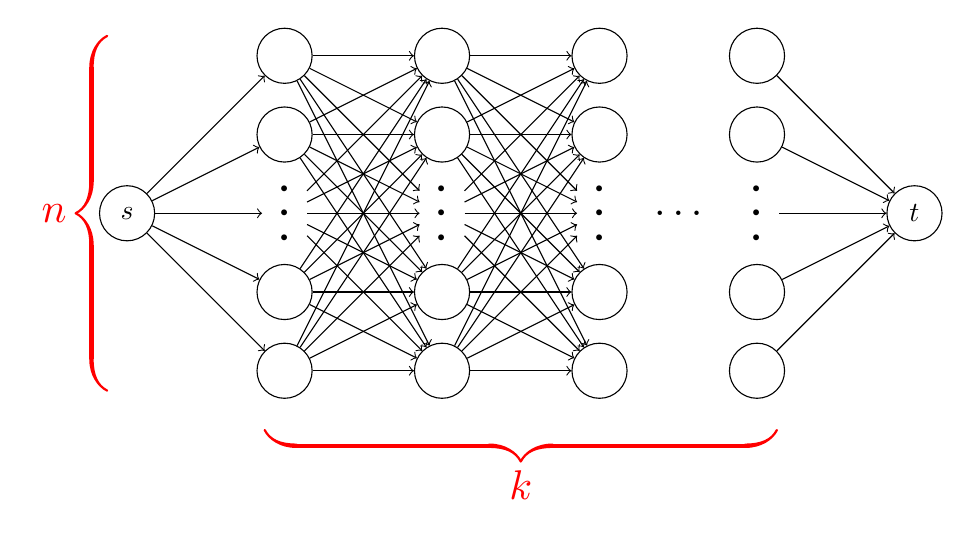
\begin{tikzpicture}
\node[draw, circle, minimum size=0.7cm] (s) at (0, 0) {$s$};
\node[draw, circle, minimum size=0.7cm] (t) at (10, 0) {$t$};

\node[draw, circle, minimum size=0.7cm] (l1v1) at (2, 2) {};
\node[draw, circle, minimum size=0.7cm] (l1v2) at (2, 1) {};
\node[draw, circle, minimum size=0.7cm] (l1v3) at (2, -1) {};
\node[draw, circle, minimum size=0.7cm] (l1v4) at (2, -2) {};
\path (l1v2) -- node[scale=2, rotate=90] (more1) {$\ldots$} (l1v3);

\node[draw, circle, minimum size=0.7cm] (l2v1) at (4, 2) {};
\node[draw, circle, minimum size=0.7cm] (l2v2) at (4, 1) {};
\node[draw, circle, minimum size=0.7cm] (l2v3) at (4, -1) {};
\node[draw, circle, minimum size=0.7cm] (l2v4) at (4, -2) {};
\path (l2v2) -- node[scale=2, rotate=90] (more2) {$\ldots$} (l2v3);

\node[draw, circle, minimum size=0.7cm] (l3v1) at (6, 2) {};
\node[draw, circle, minimum size=0.7cm] (l3v2) at (6, 1) {};
\node[draw, circle, minimum size=0.7cm] (l3v3) at (6, -1) {};
\node[draw, circle, minimum size=0.7cm] (l3v4) at (6, -2) {};
\path (l3v2) -- node[scale=2, rotate=90] (more3) {$\ldots$} (l3v3);


\node[draw, circle, minimum size=0.7cm] (l4v1) at (8, 2) {};
\node[draw, circle, minimum size=0.7cm] (l4v2) at (8, 1) {};
\node[draw, circle, minimum size=0.7cm] (l4v3) at (8, -1) {};
\node[draw, circle, minimum size=0.7cm] (l4v4) at (8, -2) {};
\path (l4v2) -- node[scale=2, rotate=90] (more4) {$\ldots$} (l4v3);

\path (more3) -- node[scale=1.5] {$\ldots$} (more4);

\foreach \v in {l1v1, l1v2, more1, l1v3, l1v4}
    \draw[->] (s) -- (\v);

\foreach \v in {l4v1, l4v2, more4, l4v3, l4v4}
    \draw[->] (\v) -- (t);

\foreach \u in {l1v1, l1v2, more1, l1v3, l1v4}
    \foreach \v in {l2v1, l2v2, more2, l2v3, l2v4}
        \draw[->] (\u) -- (\v);

\foreach \u in {l2v1, l2v2, more2, l2v3, l2v4}
    \foreach \v in {l3v1, l3v2, more3, l3v3, l3v4}
        \draw[->] (\u) -- (\v);


% Annotate parameters
\draw[decorate, decoration={calligraphic brace, mirror, raise=0.5cm, amplitude=0.4cm}, ultra thick, pen colour={red}] (l1v4.south west) -- (l4v4.south east) node[pos=0.5, below=0.8cm, red, scale=1.5]{$k$};

\draw[decorate, decoration={calligraphic brace, mirror, raise=2cm, amplitude=0.4cm}, ultra thick, pen colour={red}] (l1v1.north west) -- (l1v4.south west) node[pos=0.5, left=2.3cm, red, scale=1.5]{$n$};
\end{tikzpicture}
    \caption{Network flow stress test architecture}
    \label{fig:stress-test-architecture}
\end{figure}

We then prompt our implementation to solve the maximum flow problem against this randomly generated flow network. Validating the solution generated requires checking that flows are non-negative, that flow is conserved, and that a maximum flow was generated. The first two conditions are straightforward to check. Checking the last condition can be done by implementing the Ford-Fulkerson method and seeing if the linear program solution matches that of the Ford-Fulkerson method. While this works, we would run into another conundrum involving the validation of the Ford-Fulkerson implementation. To reduce implementation complexity, we instead opted into exploiting the Max-Flow Min-Cut Theorem. The theorem says that we can verify a maximum flow by checking if the residual network associated with a flow has no augmenting paths. In fact, the converse also holds making this check both sound and complete. Therefore, to check if our solver successfully found a maximum flow, we construct the associated residual network for the flow generated and check if there exists no augmenting paths using a depth-first-search. 

\section{Discussion}
In this report, we discussed our implementation of the simplex algorithm and how it solves linear programming problems. We modeled our implementation after that in \cite{CLRS} but made a few additional contributions. In particular, we implemented an easy-to-use interface to construct linear programs that does not require deep knowledge of linear programming. We provided sketches of our implementation's design along with the rationale behind some of our design choices. These design choices led us to present the obstacles we faced during implementation along with subtle issues obscured when considering the simplex algorithm in the abstract. We also showed our validation methods to gain confidence in our implementation's robustness. In particular, we presented a novel testing method based on randomly generated maximum flow problems and showed how one can quickly verify a solution without having to actually solve the original maximum flow problem using the Max-Flow Min-Cut Theorem. 

For the details of our implementation, please see \url{https://github.com/EthanTheMaster/LinearProgrammingSimplexAlgorithm} which hosts our implementation.

\bibliography{refs}
\end{document}
